%!TEX root=../../../root.tex

Learning is about discovering a \emph{map} from input to output. Finding a model explaining the data means determining the map.
The key assumption that we are going to use is that data has an \emph{underlying structure}; however, it is very infrequent that this structure can be captured by a simple expression.

\paragraph{Choosing a representation}
The same data can be described in different ways, take for example the following curve
\begin{figure}[H]
	\centering
	\includegraphics[width=.3\textwidth]{02/linear}
	\caption{A linear curve.}\label{fig:linear}	
\end{figure}
this curve can be represented as a \emph{function} with 2 weights
\begin{equation}
	y = ax + b
\end{equation}
or as a \emph{parametric curve} with 4 weights:
\begin{equation}
	\begin{pmatrix}x\\y\end{pmatrix} = \begin{pmatrix}a_x\\a_y\end{pmatrix}t+\begin{pmatrix}b_x\\b_y\end{pmatrix}.
\end{equation}
in the former, each datapoint is the output of a function of one single number $x$; in the latter, each point is modeled as a pair of numbers $(x,y)$ linked to a variable $t$ with a linear model over $x$ and a linear model over $y$. In general, a parametric curve is a normal curve where we choose to define the curve's $x$ and $y$ values in terms of another variable.
In this example, $a_x = 1, b_x = 0$ so the value for $x$ is completely determined by the value of $t$, while the values of $a_y, b_y$ are those of $a,b$ of the previous formula.

\begin{figure}[H]
	\centering
	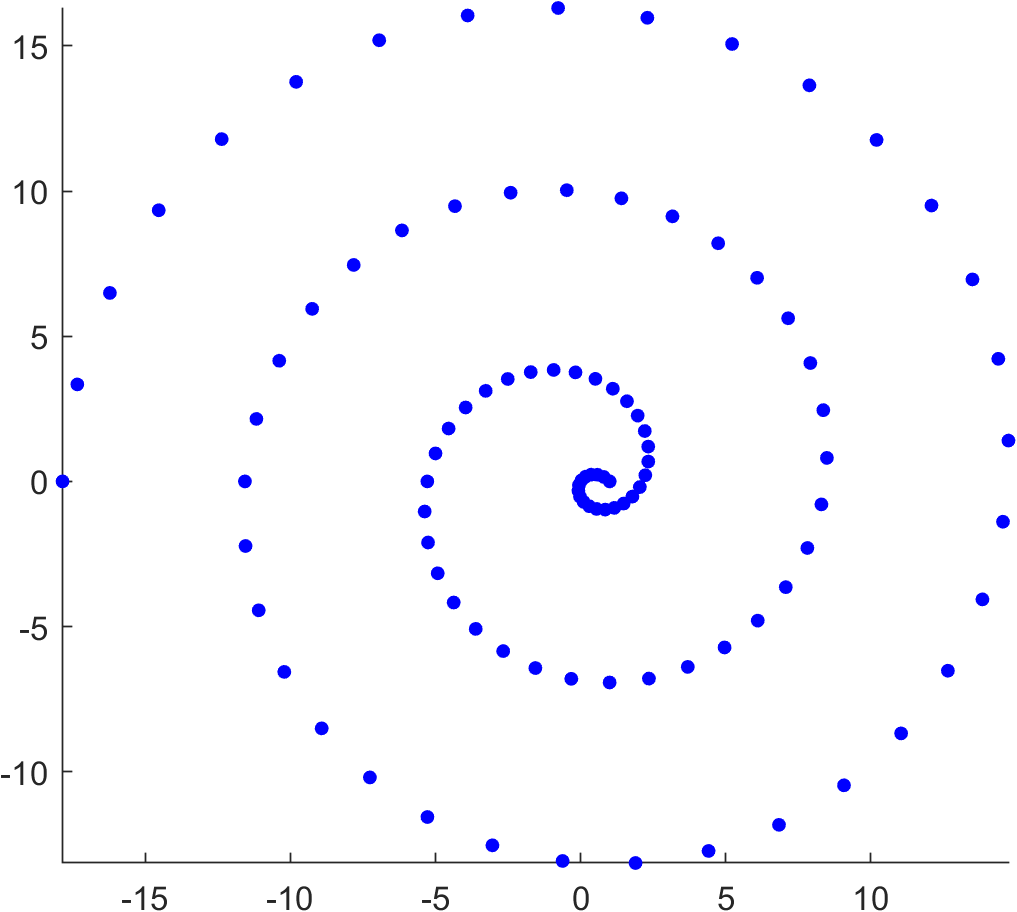
\includegraphics[width=.3\textwidth]{02/spiral}
	\caption{A spiral-shape dataset.}\label{fig:spiral}
\end{figure}

In \cref{fig:spiral} instead, it seems that there is no way to describe the given dataset with a function, but we can easily do it with a parametric curve
\begin{equation}
	\begin{pmatrix}x\\y\end{pmatrix} = a\begin{pmatrix}cos(t)\\sen(t)\end{pmatrix}(a-t).
\end{equation}
Actually, the dataset can also be described with a function, by switching to polar coordinates
\begin{equation}
	r = a\theta 
\end{equation}
which is even linear. In general, there is a trade-off between the number of weights and the simplicity of the model.